\documentclass[12pt,a4paper]{article}
\usepackage{fullpage}
\usepackage[utf8]{inputenc}
\usepackage{amsmath}
\usepackage{amsfonts}
\usepackage{amssymb}
\usepackage{enumerate}
\usepackage{enumitem}
\usepackage{graphicx}

\setlist{nosep}

\begin{document}

%\title{CSCI 4448: Object Oriented Analysis and Design\\ Project Part 2}
%\date{October 19, 2015}        
%\maketitle

\noindent\textbf{Project Part 2}

\paragraph{Team:}Andrew Gordon, Tommy Hoffmann, Connor McGuinness, Daniel Zurawski

\paragraph{Title:}What To Wear Weather

\paragraph{Project Summary:}Most people do not care about about specifics of the weather like
temperature and humidity but are more interested in things like what clothes to wear or how
event plans may be affected. Our project is an Android application which tells users what kind
of clothes they should be wearing based on the weather in their local area while not displaying
information about the weather users are not interested in.
\\

\noindent\textbf{Requirements:}
\\\\
%insert tables here
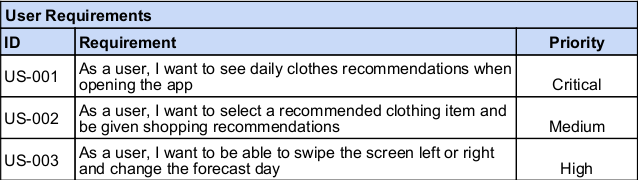
\includegraphics[scale=0.7]{user.png}\\\\
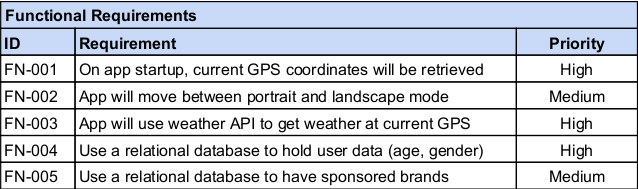
\includegraphics[scale=0.7]{functional.png}\\\\
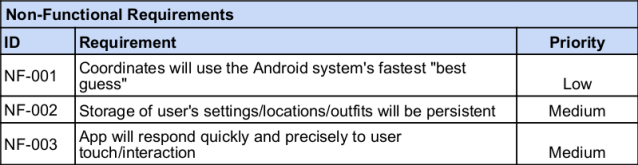
\includegraphics[scale=0.7]{non-functional.png}\\\\

\pagebreak

\noindent\textbf{Users and Tasks:} \\\\
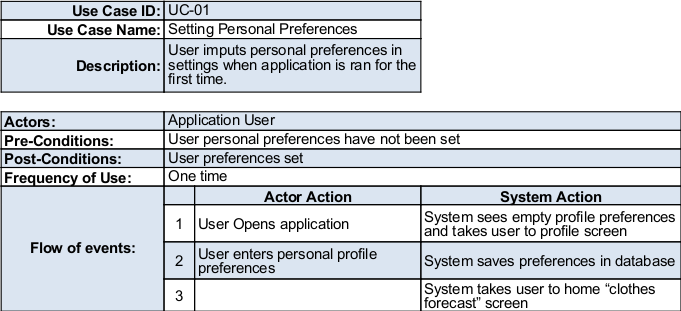
\includegraphics[scale=0.7]{usecase1.png} \\\\
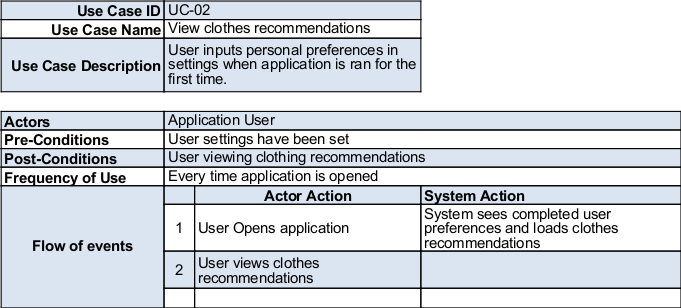
\includegraphics[scale=0.7]{usecase2.png} \\\\
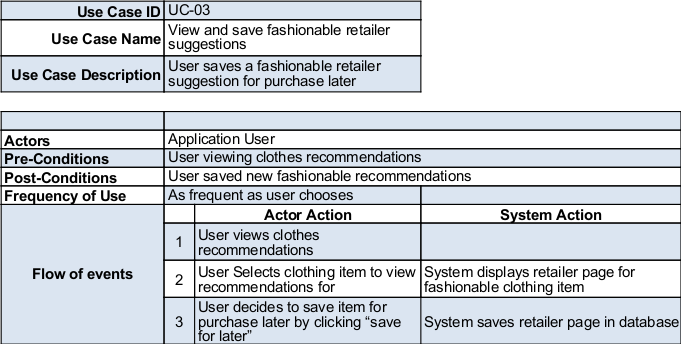
\includegraphics[scale=0.7]{usecase3.png} \\\\
%insert use case diagrams

\paragraph{Activity Diagram:}
%activity of most complex use case

\paragraph{Data Storage:} The application will use the Android internal storage in XML format.
The storage requirements are not very large, in particular user preferences and saved clothing recommendations
will needed to be stored, which we anticipate will be a few dozen items.
The User Preferences class and Clothes Recommendation class will be retrieving and modifying data from data storage.
If XML format ends up not being adequate we will use a SQL Lite database.

\paragraph{UI Mockups:} 

\paragraph{User Interaction 1:} Viewing Recommendations\\\\
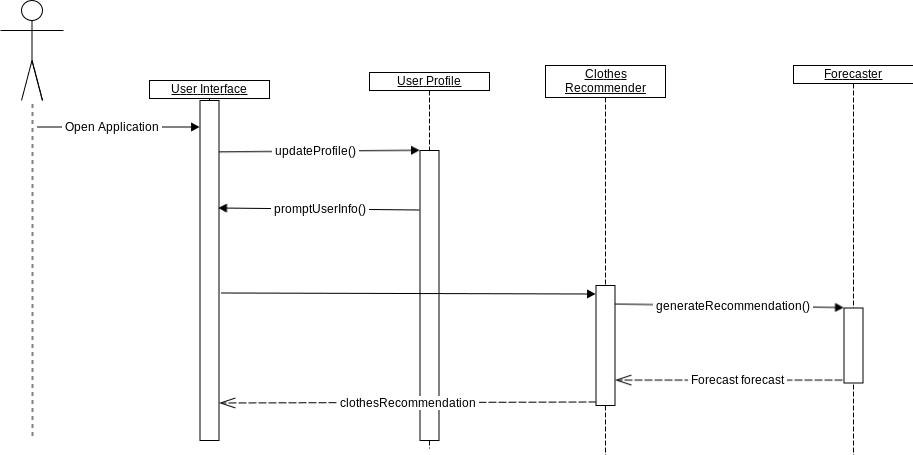
\includegraphics[scale=0.5]{us_01_veiwrecs.png}

\paragraph{User Interaction 2:} Setting Personal Preferences\\\\
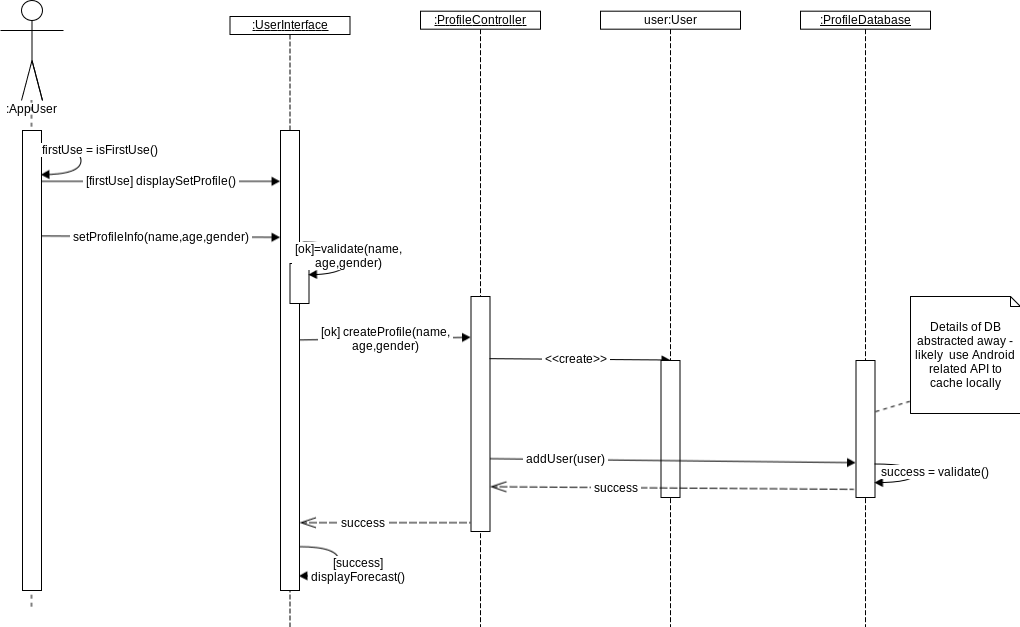
\includegraphics[scale=0.45]{uc2_settingpersonalprefssequence.png}

\paragraph{User Interaction 3:} Setting Personal Preferences\\\\
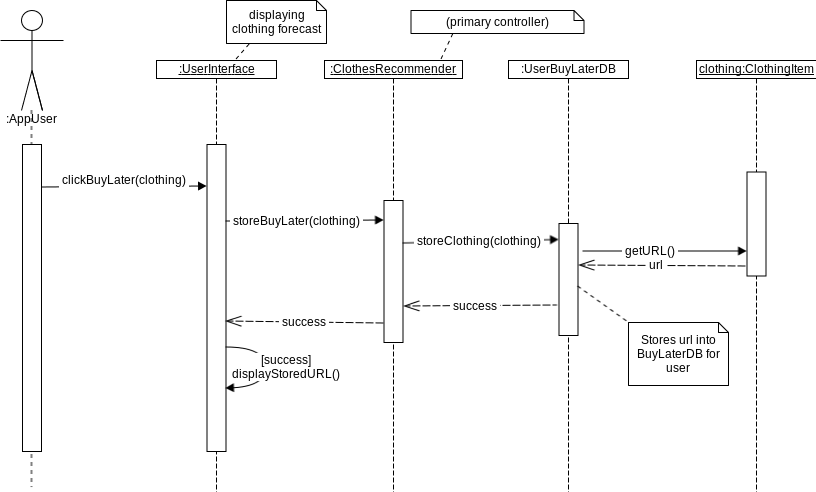
\includegraphics[scale=0.5]{uc_03_savefashionsuggestion.png}



\paragraph{Class Diagram}
\end{document}
